\chapter{Utilizzo}
Nei prossimi punti vediamo degli accorgimenti che sono utili per far utilizzare il sistema nel modo corretto. Per osservare degli esempi di come strutturare il codice osservare le sezioni di questo capitolo.
\begin{itemize}
    \item Gli elementi del sistema, come task, taskset e scheduler, devono essere definiti all'interno del main. Una volta definito tutto si deve chiamare il metodo \texttt{schedule} sullo scheduler. Nel caso si voglia generare una sorta di dataset di tracce, è prevista la possibilità di chiamare più volte il metodo \texttt{schedule} all'interno dello stesso main. Per generare un dataset di tracce è invece necessario chiamare il metodo \texttt{scheduleDataset} passando come parametro il numero di tracce.
    \item Un task campiona il suo tempo di esecuzione da una distribuzione. Tale distribuzione, passata come parametro del costruttore, è un oggetto di tipo \texttt{Sampler} definito nella libreria Sirio. Oltre alle distribuzioni introdotte da Sirio è presente anche l'implementazione \texttt{ConstantSampler}, che definisce un campionamento costante.
    \item I tempi devono essere passati al sistema e letti da esso in millisecondi. Il sistema li gestisce in nanosecondi per avere un'alta precisione.
\end{itemize}
Per concludere analizziamo come il sistema si comporta sulla generazione di dataset. Si procederà in modo incrementale, per capire come affrontare lo scheduling di taskset più semplici e poi quelli più complessi.

Questa parte può essere anche utile per capire come strutturare il main ed utilizzare il simulatore.

%%%%%%%%%%%%%%%%%%%%%%%%%%%%%%%%%%%%%%%%%%%%%%%%%%%%%%%%%%%%%%%%
\section{Baseline}
Vediamo come funziona una simulazione tramite RM con un taskset molto semplice. Il taskset in questione, come si può notare dal codice in Figura~\ref{fig:baselineTaskset}, è molto semplice in modo da poter osservare le differenze tra le due simulazioni. Si tratta di un taskset con due task puramente periodici: il primo ha periodo e deadline relativo pari a 20ms e un execution time di 10ms; il secondo ha periodo e deadline di 60ms e un execution time di 12ms.

La traccia in Figura~\ref{fig:baselineTrace} è l'output della simulazione.

\begin{figure}[htbp]
    \centering
    \begin{subfigure}{0.45\textwidth}
        \vfill
        \centering
        \raisebox{7em}{
            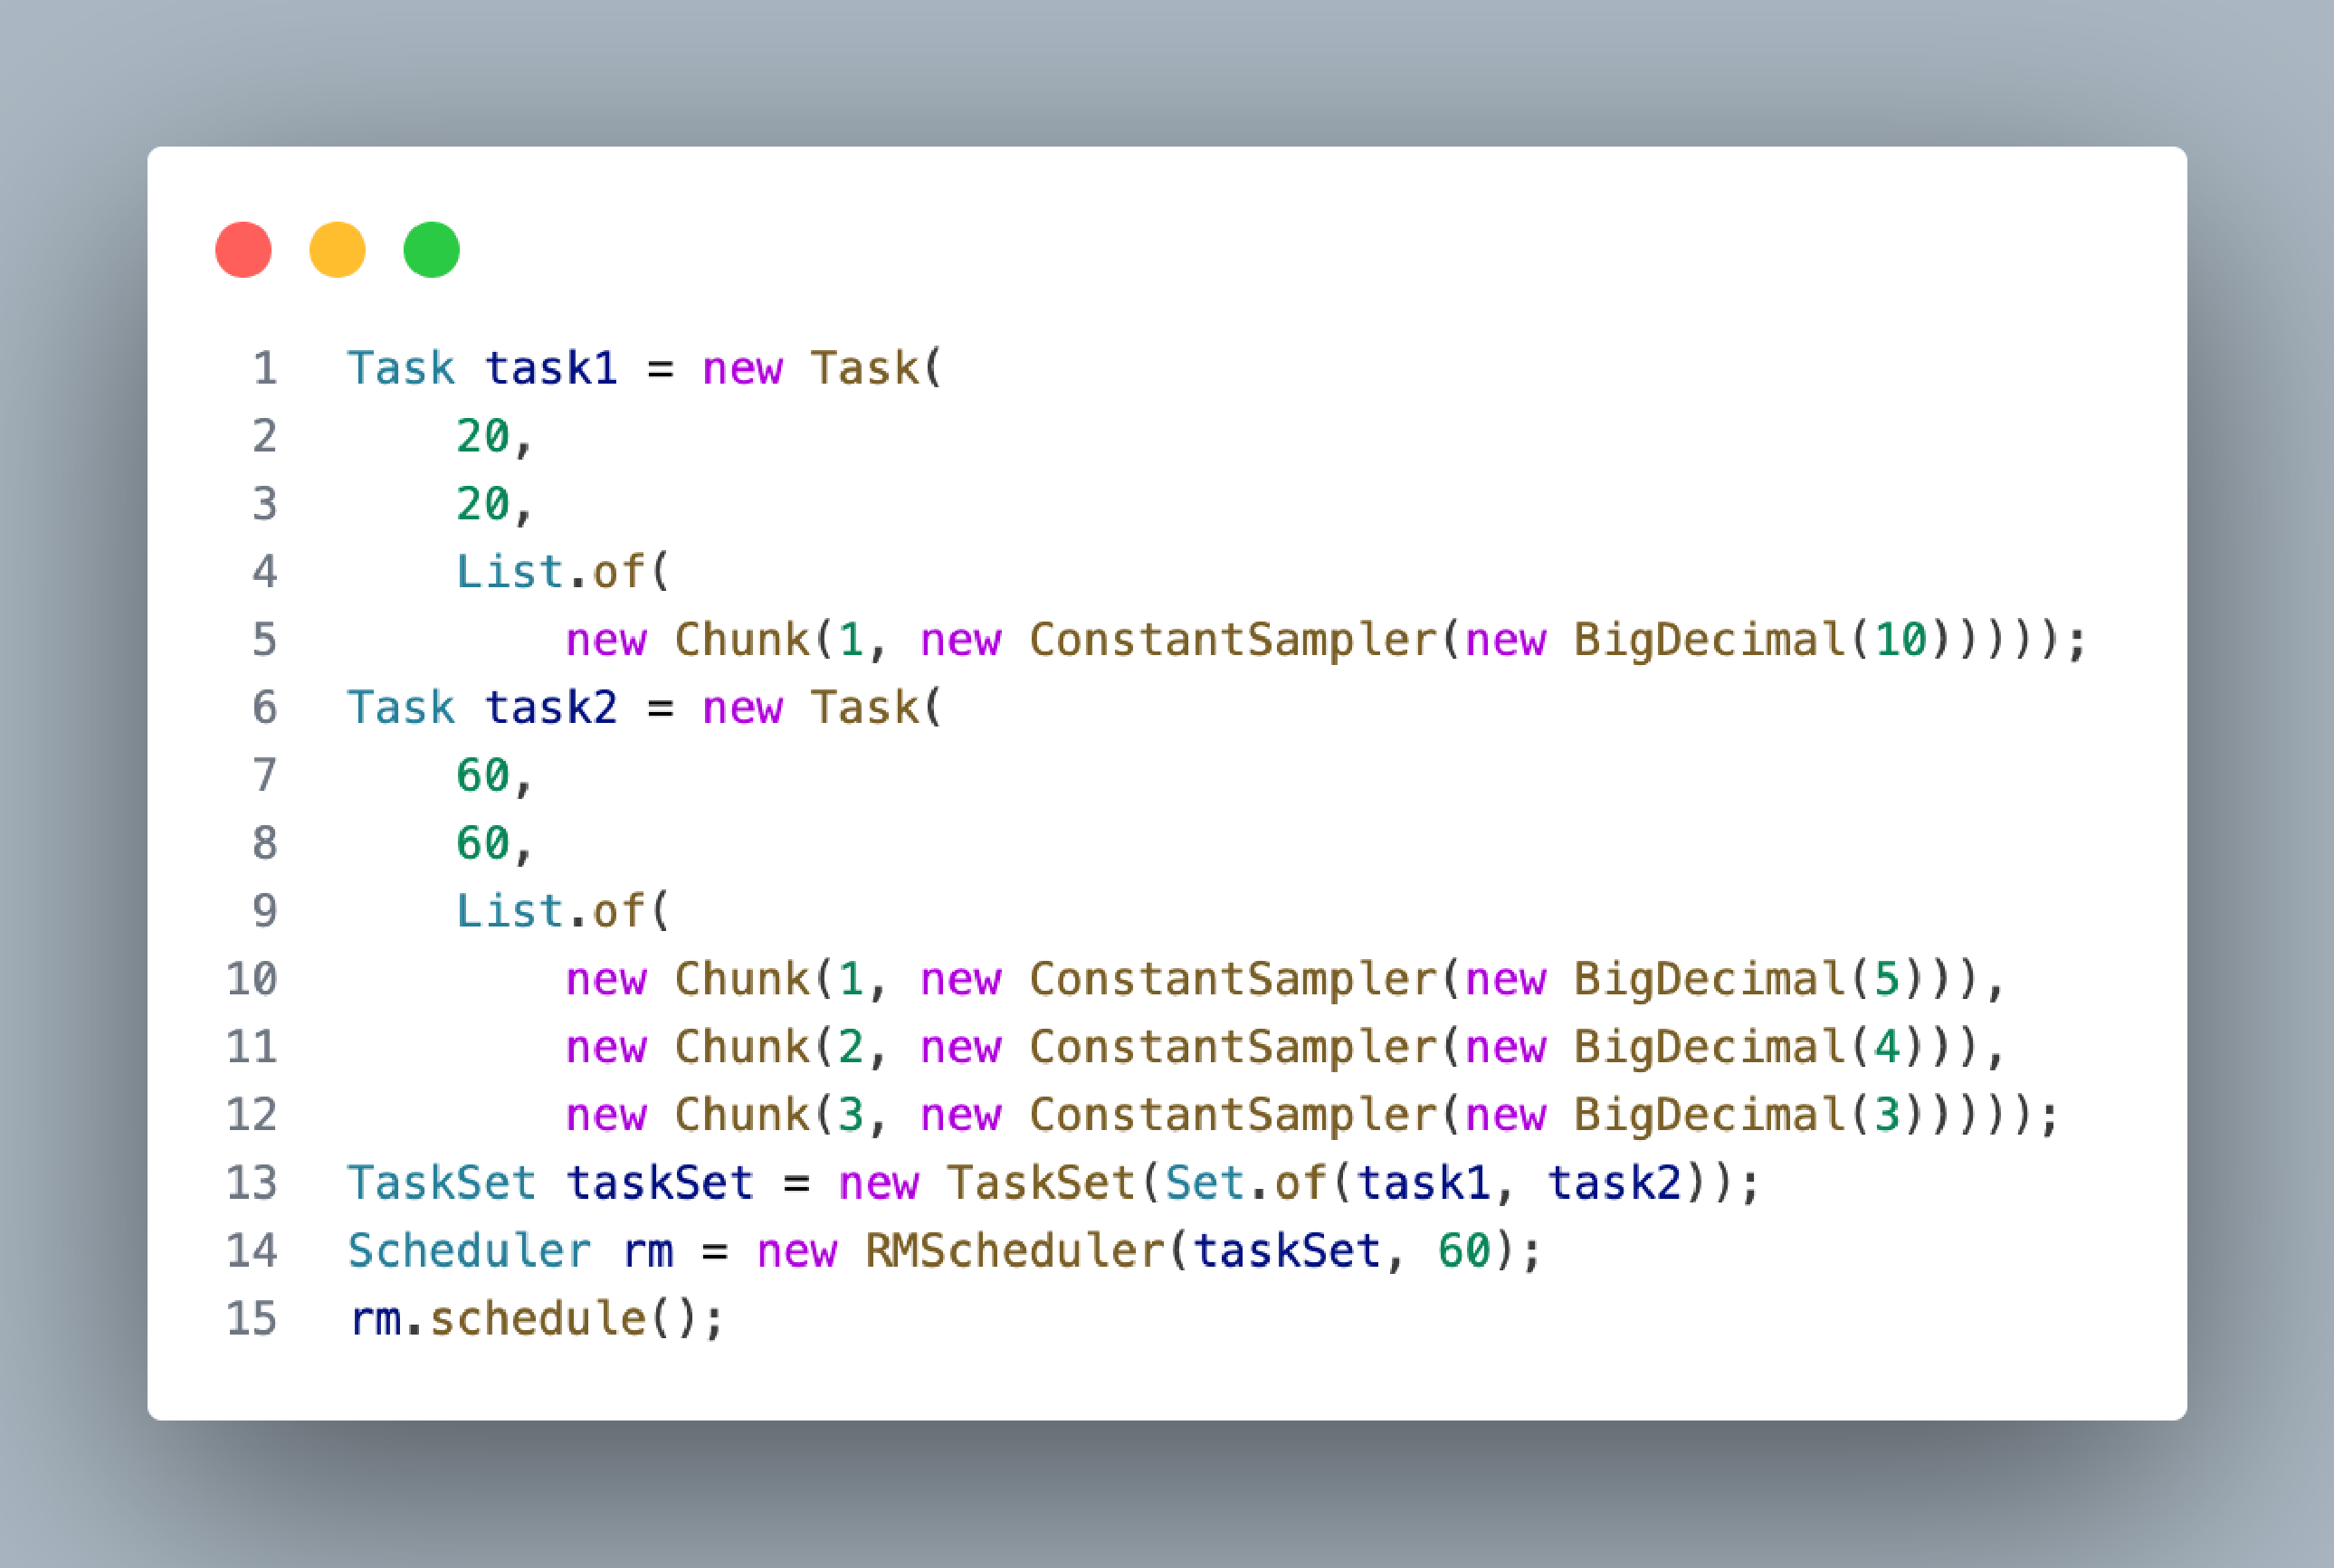
\includegraphics[width=.9\textwidth]{immagini/taskset baseline.pdf}
        }
        \caption{Taskset della baseline}
        \label{fig:baselineTaskset}
        \vfill
    \end{subfigure}
    \hfill
    \begin{subfigure}{0.45\textwidth}
        \vfill
        \centering
        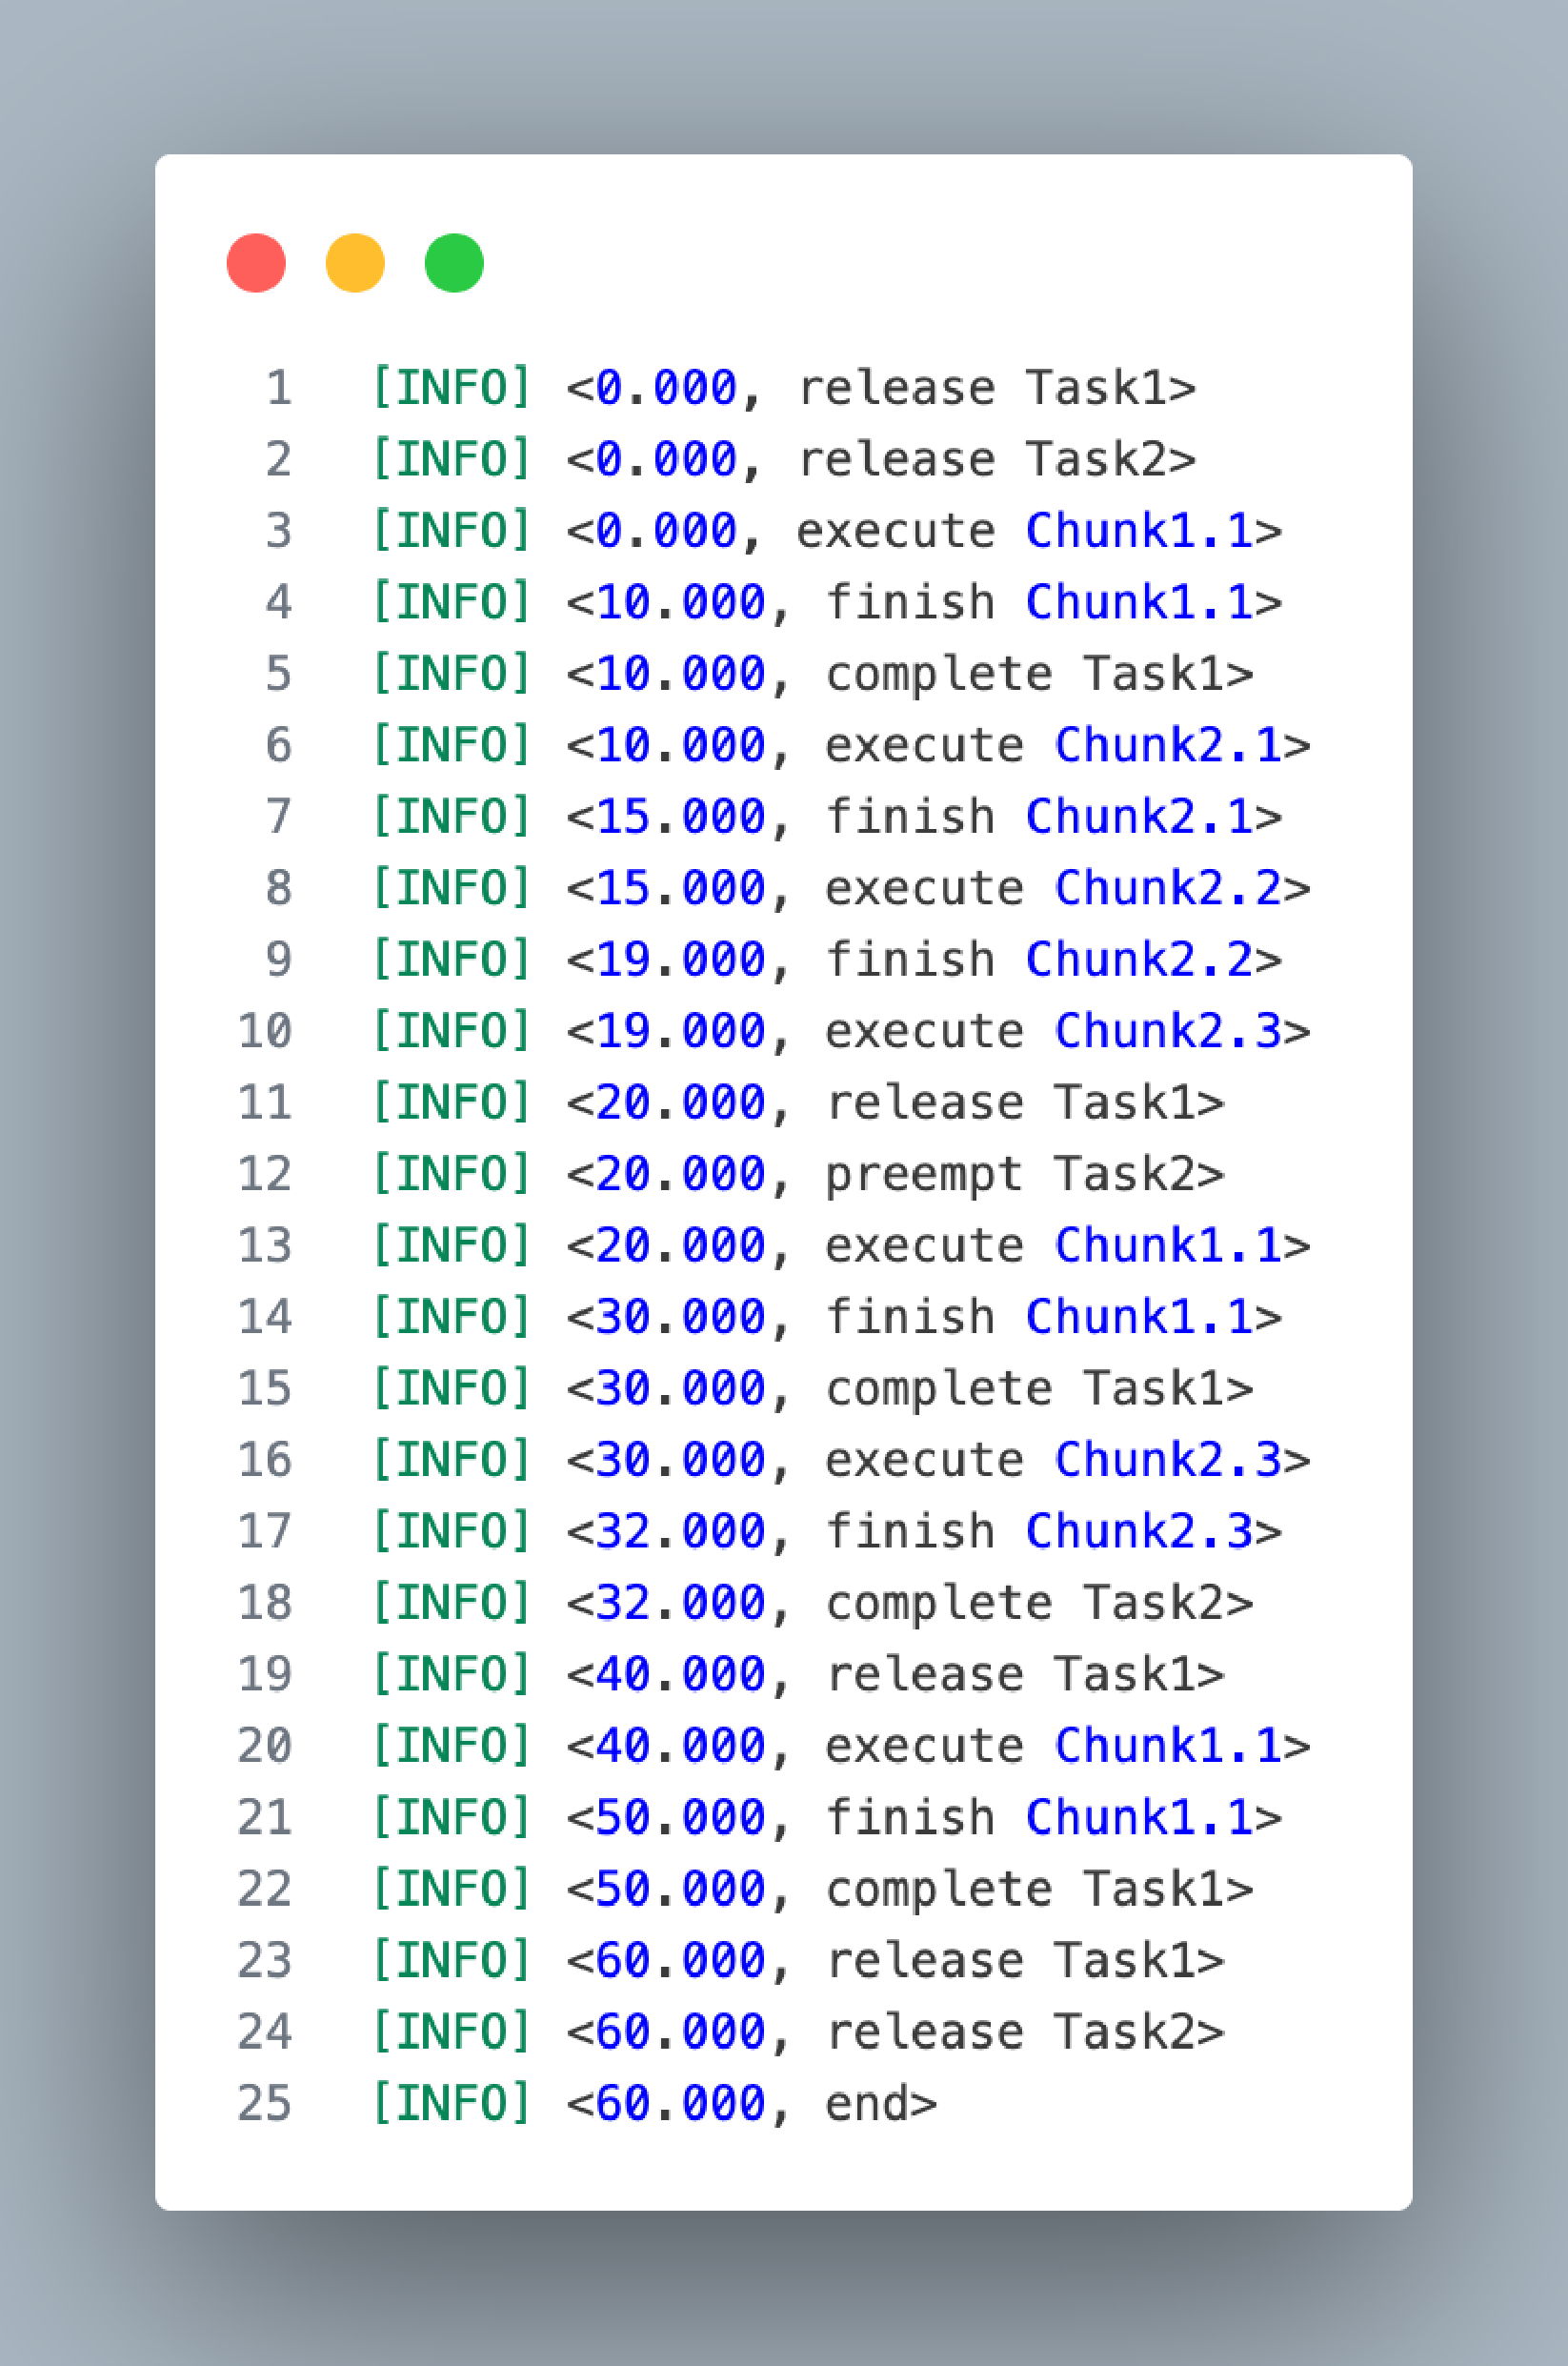
\includegraphics[width=.9\textwidth]{immagini/trace baseline.pdf}
        \caption{Traccia della baseline}
        \label{fig:baselineTrace}
        \vfill
    \end{subfigure}
    \caption{Baseline.}
\end{figure}